\chapter{Design}
\label{chap:design}

\section{Overview}
\label{sec:designintroduction}

In this chapter, we describe the architecture of the Socrates Sim framework, highlight key design choices, and describe in detail the component parts. Our goal is to develop a modularized and production-grade dialog simulation framework that can be re-targeted for new domains, produce training data and evaluate dialog agents. The overall design for the simulator was inspired by the work done by \cite{li_usersim}. For the user simulator, we implement the theoretical formulation of the hidden user agenda models described by \cite{Schatzmann2009TheHA}. We also adopt the configuration first user access pattern used in the AllenNLP library \cite{Gardner_allennlp}.

At a high level, Socrates Sim consists of the following components:
\begin{itemize}
	\item \textbf{Dialog Domain}: A set of classes to represent the dialog domain and knowledge base. The dialog domain consists of all possible dialog acts, valid inform/request slots and values, and other domain-specific information. 
	\item \textbf{Speaker Interface}: A unified interface that defines a standardized protocol for the external user simulators and dialog agent to communicate with the framework. 
	\item \textbf{Dialog Manager}: A coordinator tool that facilitates the conversation between the user simulator and dialog agent. Additionally, the dialog manager tracks simulation histories, evaluates simulated dialogs, and serializes annotated dialogs to disk.  
\end{itemize}


\section{Architecture and Design} 

The general architectural is greatly inspired by the end-to-end neural dialog framework described in \cite{li_end_to_end}  (see Figure \ref{fig:li_end_end}). In this design, there are two key components. The first is an agenda based user simulator, which has an internal natural language generation (NLG) model. The right-hand side of the framework is the Neural Dialog System, which consists of a language understanding (LU) unit and a dialog management (DM) unit. The user simulator generates speech utterances using its NLG and sends to the LU unit. The LU parses the speech utterance into a semantic frame (implemented as Python dictionary) and hands it the dialog management unit, which generates a system action and sends to the user simulator (as a semantic frame). The dialog manager also has a state tracker and policy learner. The policy learner is implemented as a deep Q-network (DQN). 

\begin{figure}[h!]
	\label{fig:li_end_end}
	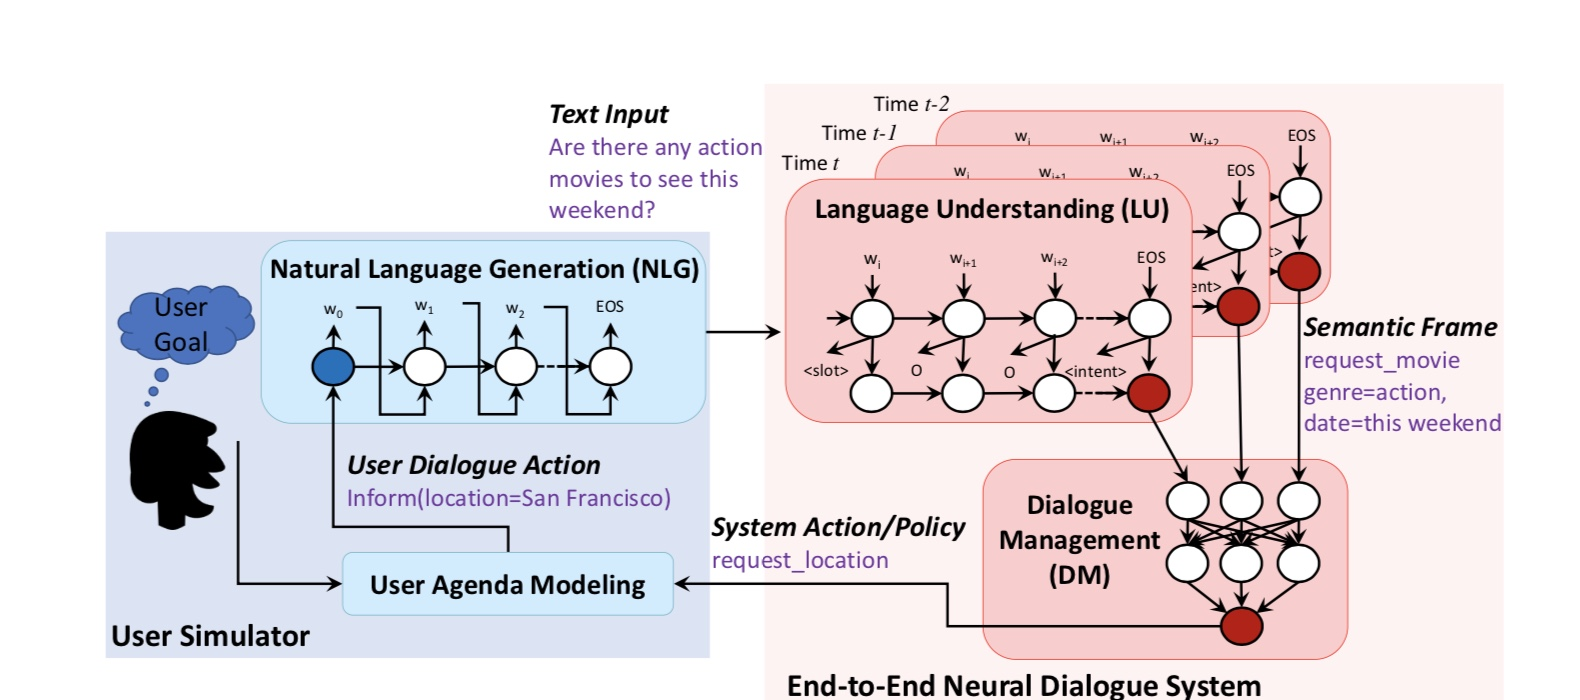
\includegraphics[width=\linewidth]{diagrams/li_end_to_end.jpeg}
	\caption{ The user simulator architecture described by Li et al. (2016) }
\end{figure}

The neural dialog system uses reinforcement learning to learn optimal policies for the dialog agent. At the end of each simulated conversation, the dialog manager will score itself and update its policy learner. One of the key limitations of this approach is that the dialog agent is built in as a learner in the Neural Dialog System. After a set of predefined rounds, the output will be a neural dialog agent serialized as a model file. The simulated dialogs will also be stored externally and can be used downstream as further training data.

The primary challenge with this framework is that it is difficult to adapt it to new domains. While the user simulator is a separate component and can be easily reconfigured, the dialog agent and dialog manager are tightly coupled. The dialog agent must be implemented as a neural learner. To adapt this framework to a new domain would require rewriting the dialog manager, language understanding unit, and the surrounding scaffolding scripts which set up and run the simulations. In the research code provided by \cite{li_end_to_end}, the domain information (movie booking) is directly hardcoded into all the aspects of the framework. Communication between components takes place with Python dictionaries, which can be defined arbitrarily. This introduces an element of variability that can present challenges downstream for debugging.

\begin{figure}[h!]
	\label{fig:socrates_sim_framework}
	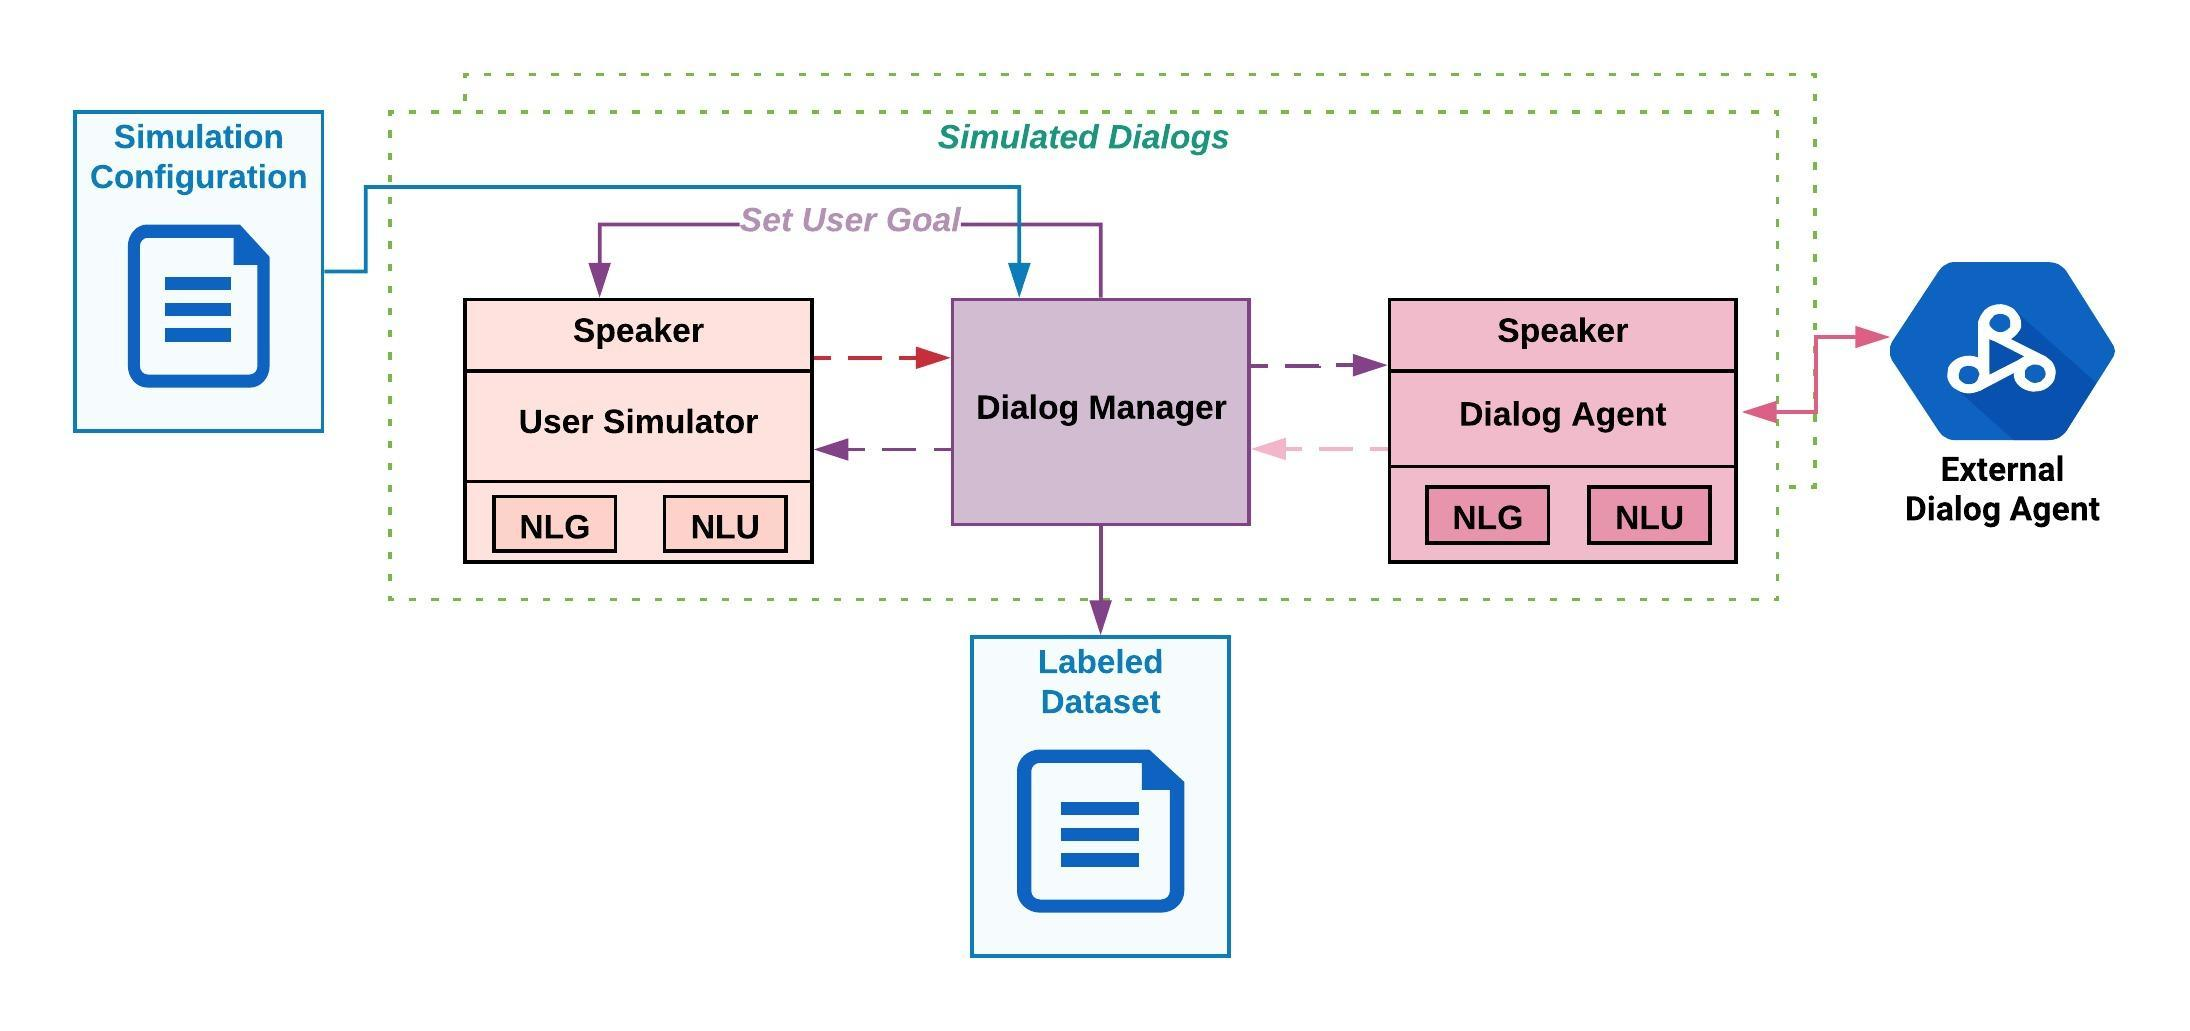
\includegraphics[width=\linewidth]{diagrams/socrates_diagram.jpeg}
	\caption{ Design of the Socrates Sim framework. }
\end{figure}

The Socrates Sim framework was designed to generalize to new domains and provide a consistent experience for dialog simulation and generation of labeled data. Figure \ref{fig:socrates_sim_framework} provides a high-level overview of the framework. The framework is simple. There are three key modules, the user simulator, the dialog agent, and the dialog manager. We assume that the user simulator and dialog agent have been implemented externally. In order to fit into the framework, they need to be integrated into implementations of the \textit{Speaker} abstract base class. The \textit{Speaker} abstract base class provides a set of APIs that allow for the user simulator and dialog agent to communicate with the framework in a standardized way. Once the classes are created, their locations are stored in a configuration file that is used by the dialog manager to load speakers and run simulations. The external configuration file supports additional settings and configurations which allow rapid experimentation and make it easy to transition to new domains.

The framework needs to be modular so that it can be quickly adapted to support new dialog domains and experiments. Each major component of the framework is represented as a Python abstract base class. Both the user simulator and agent have the same base class (Speaker) and have their own internal nlg and nlu objects. The internal nlg and nlu objects are implementations of the \textit{NLG} and \textit{NLG} abstract base class. Additionally, communication between the speakers is standardized. Dialog actions, goals, and domain knowledge bases are all first-class objects. This is in stark contrast to the design choice of \cite{li_end_to_end}, where similar components are implemented as Python dictionaries. As first class objects, we can standardize the communication and management of these pieces and ensure more consistent behavior.

Another key distinction of Socrates Sim is that the framework is agnostic as to how the dialog agent is implemented. By decoupling the agent from the dialog manager, the researcher is free to test out different agents without having to rewrite the entire simulation framework.  The dialog agent class provides a simple interface to allow external agents to plug into the simulation framework. This also frees up the dialog manager to provide other useful services like metrics, dialog analysis, and labeled data generation.

\subsection{Configuration First Design} 

We want to provide as much flexibility and freedom to the researcher and limit what is hard-coded. I follow the configuration-first approach leveraged in the development of AllenNLP, a deep learning for NLP tool developed at the Allen Institute for Artificial Intelligence. The objective of the approach is to separate out domain-specific logic from implementation details. The configuration file stores information about the domain and domain specific implementation choices. As a result, the implementation code can be written at a higher level and be more flexible and re-targetable. 

To support a configuration-driven approach, each configurable module supports the ingestion of a user-defined yaml or json file. For smaller configuration details, the user may prefer to use the yaml format which is more human readable. The yaml format is simple and has a very low learning curve. It follows a basic key-value pair paradigm, where keys have clear semantic meaning and values can be represented in a variety of data structures. 

\begin{figure}[h!]
	\begin{lstlisting}
	# Dialog Simulation settings
	simulation_rounds: 10
	max_turns: 8
	first_speaker: usersim
	simulation_output_path: data/simulated_dialogs/
	\end{lstlisting}
	\caption{Example yaml section.}
	\label{fig:ex_yaml}
\end{figure}

Socrates Sim is a command line tool. Once the researcher has set up the user simulator and dialog agent, they can invoke the dialog manager and run simulations with the command line. At the end of the simulation, the dialog manager will output performance metrics for the dialog agent and store the generated dialogs with annotations.

The remainder of the chapter further describes in detail the different components of Socrates Sim.

\section{Dialog Domain and Domain Knowledge Base}
\label{sssec:dialog_domain}

\begin{figure}[h!]
	\centering
	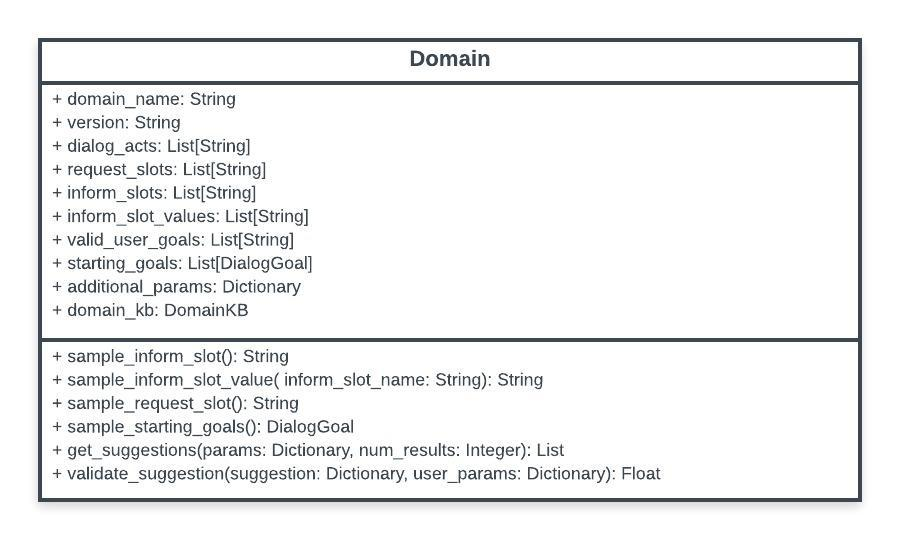
\includegraphics[scale=.9]{diagrams/domain_class.jpeg}
	\caption{ Dialog domain class. }
	\label{fig:domain_class}
\end{figure}

The domain class standardizes the collection and storage of information related to the domain of the services provided by the dialog agent. The domain class is initialized by a configuration file defined by the researcher and provides a set of APIs to access the various domain elements. The domain class consists of the following key properties: dialog acts, request slots, inform slots and inform slot values, valid user goals templates, sample starting goals list, and a domain knowledge base object.  Additionally, the following key API methods are made available: sample inform slots and inform slot values, sample request slots, get valid user goals, and get suggestions (from domain knowledge base) and validate suggestions. 

The primary consumer of the domain class is the dialog manager, which uses the domain information to generate new user goals or sample user goals from a preexisting list of starting goals. If the dialog manager is generating novel user goals, it will use the valid user goals template to create a new goal and sample the inform slots to generate the user's preferences for that goal. The domain object is also provided to the user simulator and dialog agent for use. 

The domain knowledge base (KB) is an abstract base class. Its purpose is to define a standardized way for a speaker to query and access the knowledge base. The primary purpose of the domain KB is to store all the suggestions that a dialog agent would make based on the various preferences of the user. The domain KB provides an interface with the following three methods; get suggestions, validate suggestions, and get the item. The researcher is free to use whichever back-end and implementation to resolve those three API calls. 

\begin{figure}[h!]
	\centering
	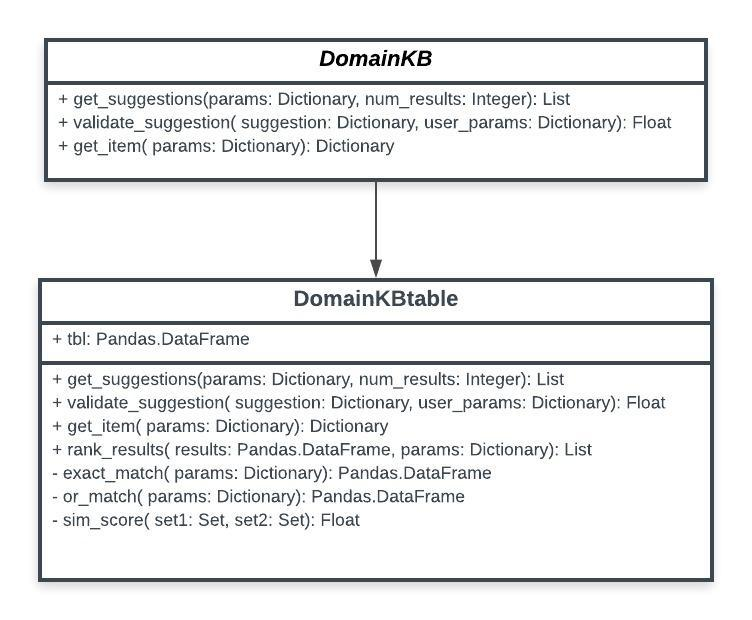
\includegraphics[scale=.8]{diagrams/domain_kb_class.jpeg}
	\caption{ Domain knowledge base abstract base class and implementation.  }
	\label{fig:domain_kb}
\end{figure}

For this thesis, \textit{DomainKBtable} is an implementation of the \textit{DomainKB} abstract base class. It loads tabular data from a csv file into a pandas data frame. The pandas data frame is a memory efficient data structure that supports querying and data manipulation. More details about the \textit{DomainKBtable} can be found in the implementation chapter. 

\section{Speaker Abstract Base Class}
\label{sssec:speaker}

The \textit{Speaker} abstract base class represents an actor that has the ability to speak and comprehend speech utterances. In our framework, both the user simulator and the dialog agent are represented by the same base speaker class. Both actors are conceptually identical in terms of functional behavior. They listen and comprehend speech utterances and respond in turn by speaking. Thus, both the user simulator and dialog agent can be represented in the same way to the dialog manager. In fact, the entire conversation round can be expressed in two lines (see Figure \ref{fig:conv_round}).

The speaker class has four basic functions (\textit{next, reset, get utterance, and parse utterance}) and three properties (\textit{nlg model, nlu model, and dialog status}). When the speaker is initialized, the nlg object and the nlu object are passed to the constructor. We abstract away the implementation of how the speaker speaks and parses speech in order to maintain separation of concerns and also empower the researcher to be able to experiment with multiple techniques. 

The \textit{next} method is the primary driver for how the speaker behaves. For the dialog agent class, the next method functions as an API to the simulator. It is assumed that the dialog agent is external to the simulator. The researcher can define how the dialog agent will interact with the user simulator here. For the user simulator, the bulk of the logic will reside here. The \textit{get utterance} and \textit{parse utterances} methods are simply wrappers for the speaker's nlg and nlu objects. The primary parameter for next is the previous dialog action. 

\begin{figure}[h!]
	\centering
	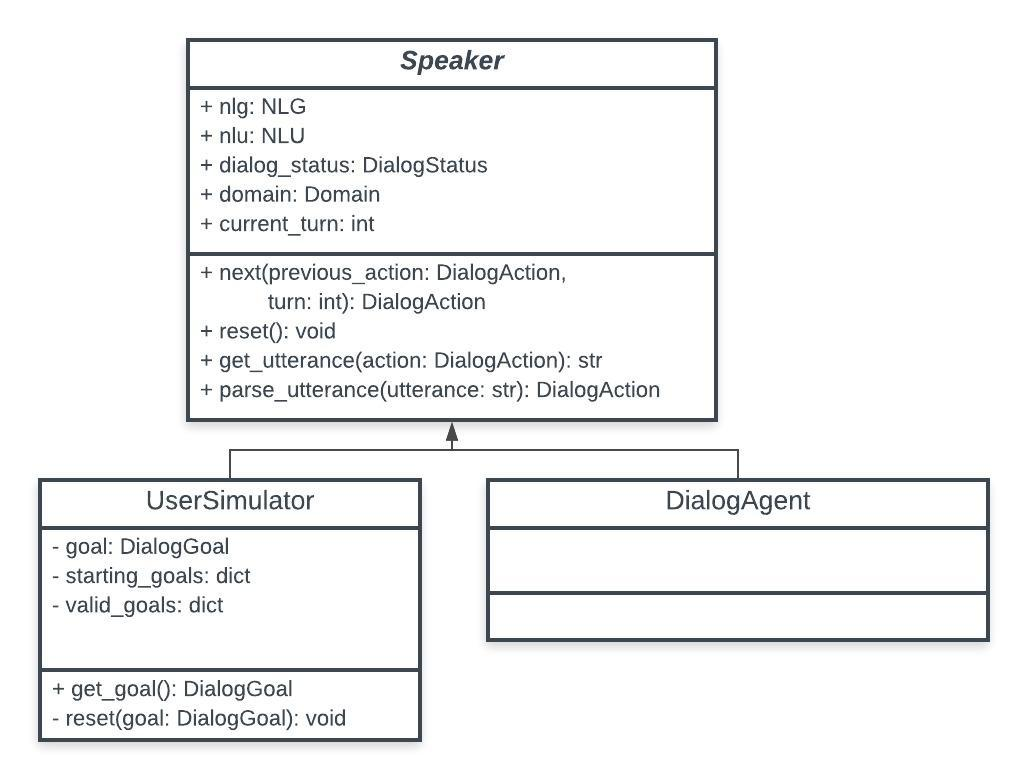
\includegraphics[width=\linewidth]{diagrams/speaker_classes.jpeg}
	\caption{ Speaker abstract base class and implementations.}
	\label{fig:speaker_class}
\end{figure}

\subsection{User Simulator}
The user simulator is responsible for imitating a real user and generating realistic speech utterances. Here we assume the user is an actor that is attempting to complete a task. For example, the user may want to travel to Japan and is attempting to book a flight there. That user could then interact with a travel agent chatbot in order to get assistance in identifying the appropriate flight and purchasing tickets. In order to model and represent a user, we will utilize the formalization of the hidden user agenda described by \cite{Schatzmann2009TheHA}.

One of the primary assumptions here is that the user has intentionally engaged with the dialog agent in order to complete their task. At the outset of the conversation, the user will have some specific goal in mind (order Indian food, book a flight to Japan, etc.). The dialog agent will attempt to learn the user's goal by asking the user a set of clarifying questions. Schatzmann and Young introduce the idea of a hidden user agenda as a mechanism to represent the sequence of dialog acts and utterances a user will say in the context of that conversation. At each step of a task-completion dialog, the user is either responding to the dialog agent or initiating a new conversation direction. The user agenda provides an efficient way and formal structure to represent the pending set of dialog acts the user will communicate to the dialog agent.

The user agenda and user goal are first class objects and are described in further detail below. Additionally, we use the \textit{UserSimulator} class (see Figure \ref{fig:speaker_class}) as an implementation of the \textit{Speaker} abstract base class. This user simulator is required to be more transparent and accessible in a particular manner by the dialog manager. At the beginning of each round, the dialog manager generates a user goal and updates the user simulator with that goal. Additionally, at the end of each conversation round, the internal state of the user simulator's goal is extracted and stored in the dialog history that is being actively tracked by the dialog manager. As a result, the researcher must implement a get\_goal and override the reset method in addition to the interface methods defined in the \textit{Speaker} abstract base class. The dialog goal is formalized as a \textit{DialogGoal} object and more details about it can be found in section \ref{sec:dialog_goal}. 

\subsubsection{User Agenda} 
~ \\
\cite{Schatzmann2009TheHA} define the user agenda as a \textit{[stack] structure of pending dialogue acts [which] serve as a convenient mechanism for encoding the dialogue history and user’s ‘state of mind’}. Formally, at any time t, the user is in a state s\textsubscript{u} and takes an action a\textsubscript{u},which transitions into an intermediate state s$'$\textsubscript{u}. During this intermediate state, the user will receive an action from the system (machine), which will transition the dialog to next state s$''$ \textsubscript{u} and the cycle will reset. The result is a sequence of alternating turns between the user and system (i.e. s\textsubscript{u} $\rightarrow$ a\textsubscript{u} $\rightarrow$ s$'$\textsubscript{u} $\rightarrow$ a$'$\textsubscript{u} $\rightarrow$ s$''$\textsubscript{u} $\rightarrow$ \dots), which represents the conversation state over time \textit{t}.

The user agenda is a stack-like structure which contains all pending user actions. User actions are actualized through popping the stack and the agenda is updated by pushing back onto the stack. A user action is a representation of the user’s intent, which will eventually be translated into a speech utterance. The stack may also contain other actions that will affect the user when popped. For example, the system can communicate a restaurant suggestion, which would fill one of the request slots with the restaurant name.  

At the start of the dialog, a new goal is randomly generated from the provided dialog domain. An accompanying agenda is then generated to represent the potential sequential of events. 

Below is an example of the sample user agenda that Schatzmann and Young provide in the context of a user asking the dialog system for a bar recommendation [6]. The states of the conversation are indexed by time t. Note, Schatzmann and Young use constraints C, which would be the equivalent of inform slots in our representation. In the first turn, the user simulator generates a set of constraints C\textsubscript{0} (bar serving beer in central) and goals (name, address, and phone for a bar that meets the constraints in C\textsubscript{0}). This set of inform and request slots are translated into a user action stored in A\textsubscript{0}. When the system initiates the conversation, the user simulator pops two inform actions which translate into the user utterance \textit{I’m looking for a nice bar serving beer}. When the system at \textit{t}=1, responds \textit{Ok, a wine bar. What price range?} the agenda is updated to include a new inform intent (inform(prange=cheap)). Also added is a negate action, as the user asked beer and not wine. 

\begin{figure}[h!]
	\centering
	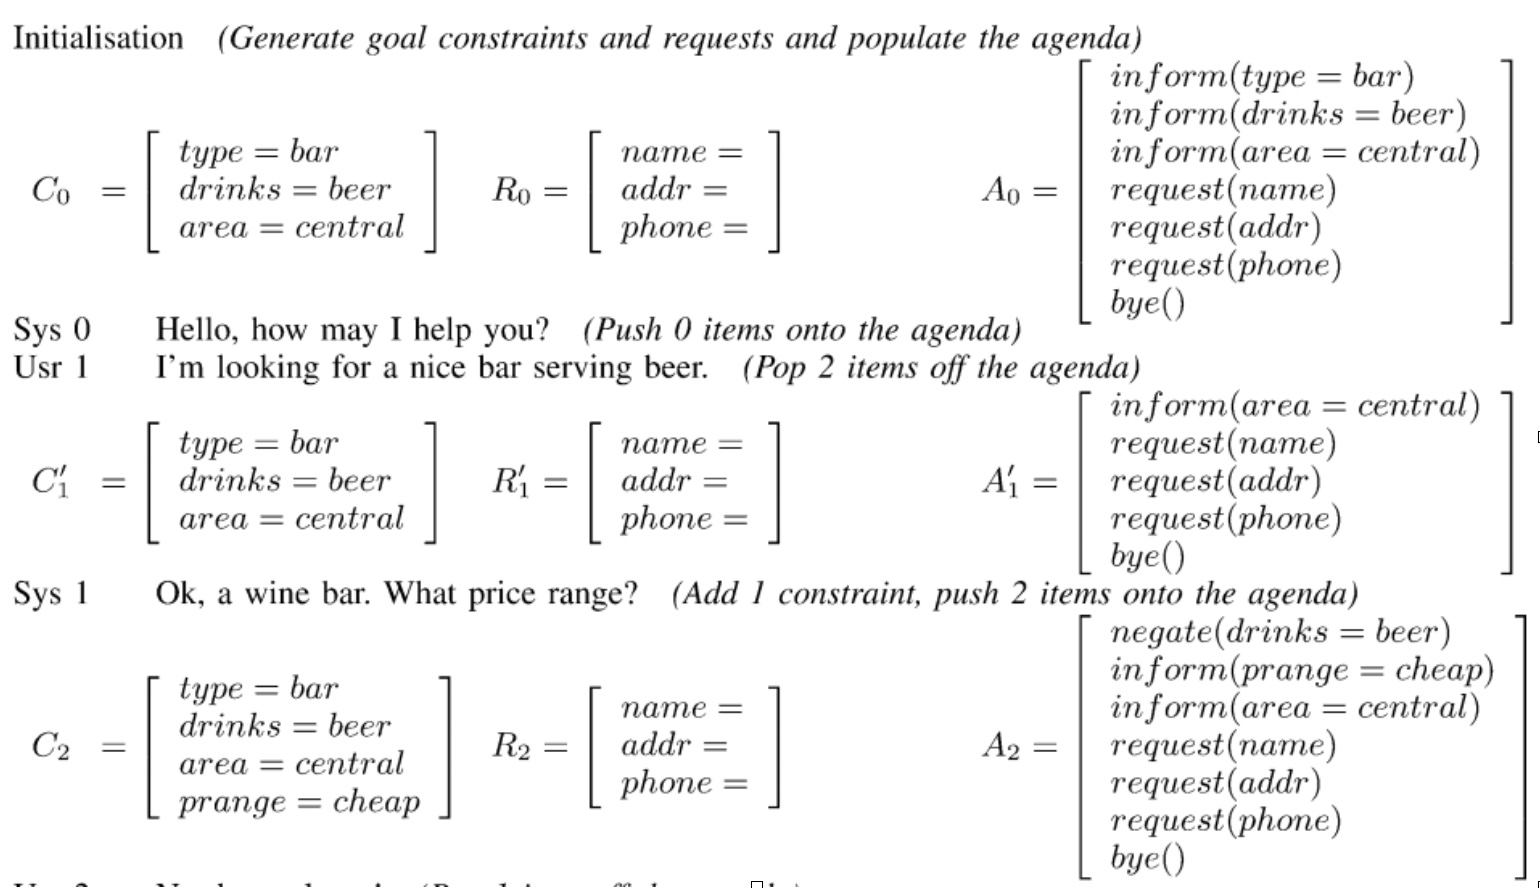
\includegraphics[scale=.25]{diagrams/ageda_ex2.jpeg}
	\caption{ Example of user agenda formulation from \cite{Schatzmann2009TheHA} }
	\label{fig:speaker_class}
\end{figure}

Over the course of the conversation, the agenda is updated, as are the request slots. The conversation ends at t=5 when bye() is popped and the agenda stack is empty. The conversation will then be evaluated based on how well the request slots were filled.

\subsection{Dialog Agent}
The framework assumes that the dialog agent is opaque and can only communicate with the framework through dialog action objects. Therefore the \textit{DialogAgent} class in Figure \ref{fig:speaker_class} serves more as a template for implementation. Implementing the four methods defined in the \textit{Speaker} abstract base class allows for the dialog agent to communicate with the dialog manager. We explore the implementation details in Section \ref{sec:speake_interface} for the \textit{DialogAgent} class.

\section{Key Dialog Components}
In order to standardize communication, we have formalized the concepts of dialog action, dialog goal, and the nlu and nlg processes. In the sections below, we investigate them in further detail.

\subsection{Dialog Action}
\label{sssec:dialog_action}

\begin{figure}[h!]
	\centering
	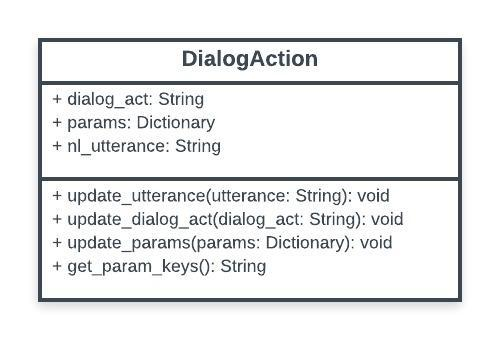
\includegraphics[scale=1]{diagrams/dialog_action.jpeg}
	\caption{ Dialog action class. }
	\label{fig:dialog_action_class}
\end{figure}

The fundamental unit of transaction for the simulator is the dialog action. It is an explicit semantic representation of the speech utterance that is machine readable. For example, I could represent the speech utterance, \textit{I'm looking for a Thai restaurant}, in the following way: \\
\textbf{original utterance}: \textit{I'm looking for a Thai restaurant}   \\
\textbf{dialog act}: \textit{request}\\ 
\textbf{constraints}: \textit{cuisine=Thai}\\

The \textit{DialogAction} object encodes information about a speech act in a standardized way. The dialog action consists of three key properties: the dialog act, a set of explicit dialog parameters or constraints, and the corresponding unparsed speech utterance. I will next describe these properties in further detail. 

The unparsed speech utterance is just the natural language utterance that was spoken by the speaker One of the objectives of the user simulator is to generate speech utterances based on its internal agenda. The user simulator will use the dialog act and dialog parameters popped from the user agenda in order to generate a new utterance using its natural language generation model. If a speaker is hearing the utterance, then the utterance will need to be parsed and broken into a dialog action and set of parameters. 

The dialog act property is used to capture the intent of the speech act. Common dialog acts include: inform, request, confirm, negate, and affirm. The dialog act is necessary to provide context for the dialog parameters for both the natural language generation and language understanding use cases. For example, a set of dialog parameters like \textit{{cuisine=thai, area=north}} can be interpreted differently in the inform vs request context. In the request context, the speech utterance could be I\textit{'d like to find a Thai restaurant in the north part of town.} In contrast, those same dialog parameters could be part of a suggestion in the inform context, e.g., \textit{There is a great Thai restaurant in the north part of town}. Given the variability of dialog acts and intents, the space of possible dialog acts is defined by the researcher in the dialog domain configuration file. While this limits the possible interpretations of a speech act, a reduced dialog act space is beneficial to building effective task-completion dialog agents.  

The dialog parameters property encodes entities found in the speech utterance as key-value pairs and is used to communicate or elicit the user's preferences. The key captures the entity/constraint type (e.g., cuisine, area, address, etc), while the value is used to indicate the specific constraint or entity (e.g., Thai, north, 115 Way Street, etc). The parameter property is strictly typed as a Python dictionary and therefore all keys must be associated with a value. In the context of request speech acts, the null value is used to indicate the speaker wants to elicit more information of the provided constraint type. For example, \textit{dialog\_act=request, params=\{address: NULL\}}, would be interpreted as a request for the address (e.g., \textit{What is the address?}). 

Initially, we used Python dictionaries and sets to represent the dialog parameters. However, this was sub-optimal for several reasons. First, it introduced variability and uncertainty. To capture the request parameters, we used Python sets, since the value was null and we just needed to pass along the constraints types. For all dialog actions, we had used explicit dictionaries as real values were passed along with the constraint types. However, downstream this required logic to check the class instance of the parameter variable being passed in. 

Given the dynamic nature of the dialogs being generated, the simulator was rather unstable and would randomly crash when a method expecting a dictionary received a set. By enforcing the Python dictionary type and setting null values, we were able to greatly improve stability and make debugging easier by standardizing the input into functions that consumed the \textit{DialogAction} object. 
\clearpage

\subsection{Dialog Goal}
\label{sec:dialog_goal}

The user goal captures explicitly the speaker's preferences and missing information they are trying to acquire. For example, consider a user who wants to find an Indian restaurant in Central Square for dinner. We can decompose this goal into two distinct components. The first is the user's explicit preferences. In this example, their preferred cuisine is Indian. The second component is implicit and unknown to the user. They are looking for a restaurant or more specifically the name and presumably the restaurant's phone number and address. This information is unknown but can be broken down into discrete pieces of information the user will attempt to elicit from the dialog agent as a request for more information. 

\begin{figure}[h!]
	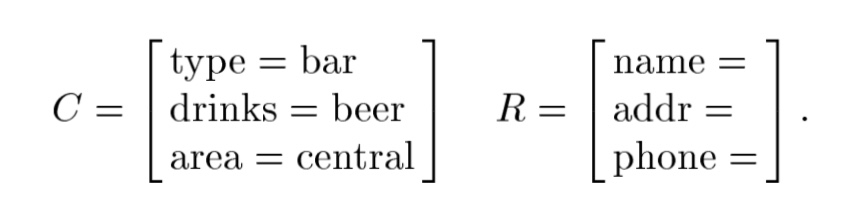
\includegraphics[scale=.35]{diagrams/schatzmann_goal_fig.jpeg}
	\caption{Example user goal. User wants the name, address and phone number of a cheap bar in central.  \cite{Schatzmann2009TheHA} }
	\label{fig:goals1}
\end{figure}

Formally, Schatzmann and Young define the user goal as \textit{G = (C,R)}, where \textit{C} consists of constraints or the user's explicit preferences and \textit{R} represents the user's requests. The constraints and requests are explicitly represented as slot-value pairs. Figure \ref{fig:goals1} above shows how one could represent the goal of a user looking for a bar. 

\begin{figure}[h!]
	\centering
	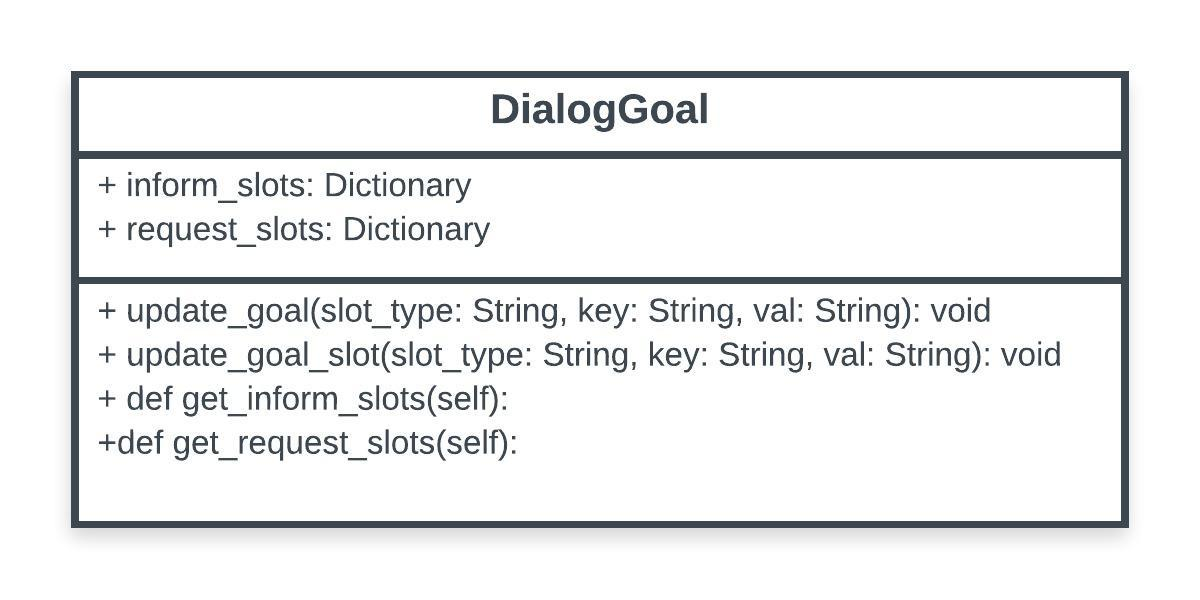
\includegraphics[scale=1]{diagrams/dialog_goal_class.jpeg}
	\caption{Dialog goal class.  }
	\label{fig:goal_class}
\end{figure}

The \textit{DialogGoal} class formalizes the Schatzmann and Young concept of the user goal. The concept of a goal abstractly turns out to be useful in also driving the dialog manager's simulations. We abstract the idea of the user goal and make it available to both the user simulator and dialog agent as a way to track the internal state of each speaker. 

For the user simulator, the goal defines the hidden set of preferences and information needs the user has. The goal object has two properties: inform slots and request slots. Both the inform and request slots are typed as Python dictionaries. The inform slots capture the user's preferences that they want to communicate to the dialog agent. A well-developed dialog agent should be able to elicit those preferences efficiently and ideally without needing to ask the user multiple times. The request slots capture the information user needs in order to complete their objective and task. At the start of the conversation, all the request slots values are set to null values. Over the course of the dialog, as the dialog agent responds the user simulator, the request slots may be updated with real values. A dialog is considered successful if all the request slots for the user simulator have been replaced by real values. The user simulator monitors the state of the request slots in it Goal object. If all the request slots are filled, the user simulator updates its internal dialog status to the complete state and signal to the dialog manager to end the conversation. 

In the first iteration, only the user simulator had the \textit{DialogGoal} object. But it made sense to allow the dialog agent to have access to its own \textit{DialogGoal} object. The rationale behind this was two-fold. First, it provides a useful mechanism to track the state of the dialog agent as well. Like the user, the dialog agent has its own set of goals, i.e. to elicit the information it needs to provide a meaningful suggestion or provide the specific service the user desires. The request slots in the dialog agent are complementary to the user's inform slots. The dialog agent can elicit the user's inform slot through a series of request speech acts and then execute its service. This leads us to the second value for the dialog agent, the \textit{DialogGoal} object provides a useful mechanism for training (especially in the reinforcement learning context). In failure cases, it signals to the researcher the information the dialog agent was ineffective in capturing. For reinforcement learning, we can develop a loss function to minimize the open request slots in the agent's \textit{DialogGoal} at the end of each conversation. 


\subsection{Dialog Status}

The \textit{DialogStatus} is a Python enumerative object that encodes the internal state of the dialog for each speaker. Each speaker is responsible for setting its own dialog status. The valid states are \textit{not started}, \textit{no outcome yet} and \textit{finished}. The dialog manager will probe each speaker for its dialog state. If the dialog manager learns that the state for any speaker is set to \textit{finished}, the conversation will be ended. The user simulator sets its dialog status to \textit{finished} when all the requests slots in its \textit{Goal} object are filled. In contrast, the dialog agent may only set its state to \textit{finished} after the user leaves the conversation. This way the agent does not prematurely exit the conversation before the user can complete their task. 

\clearpage

\subsection{NLG and NLU Abstract Base Class}


\begin{figure}[h!]
	\centering
	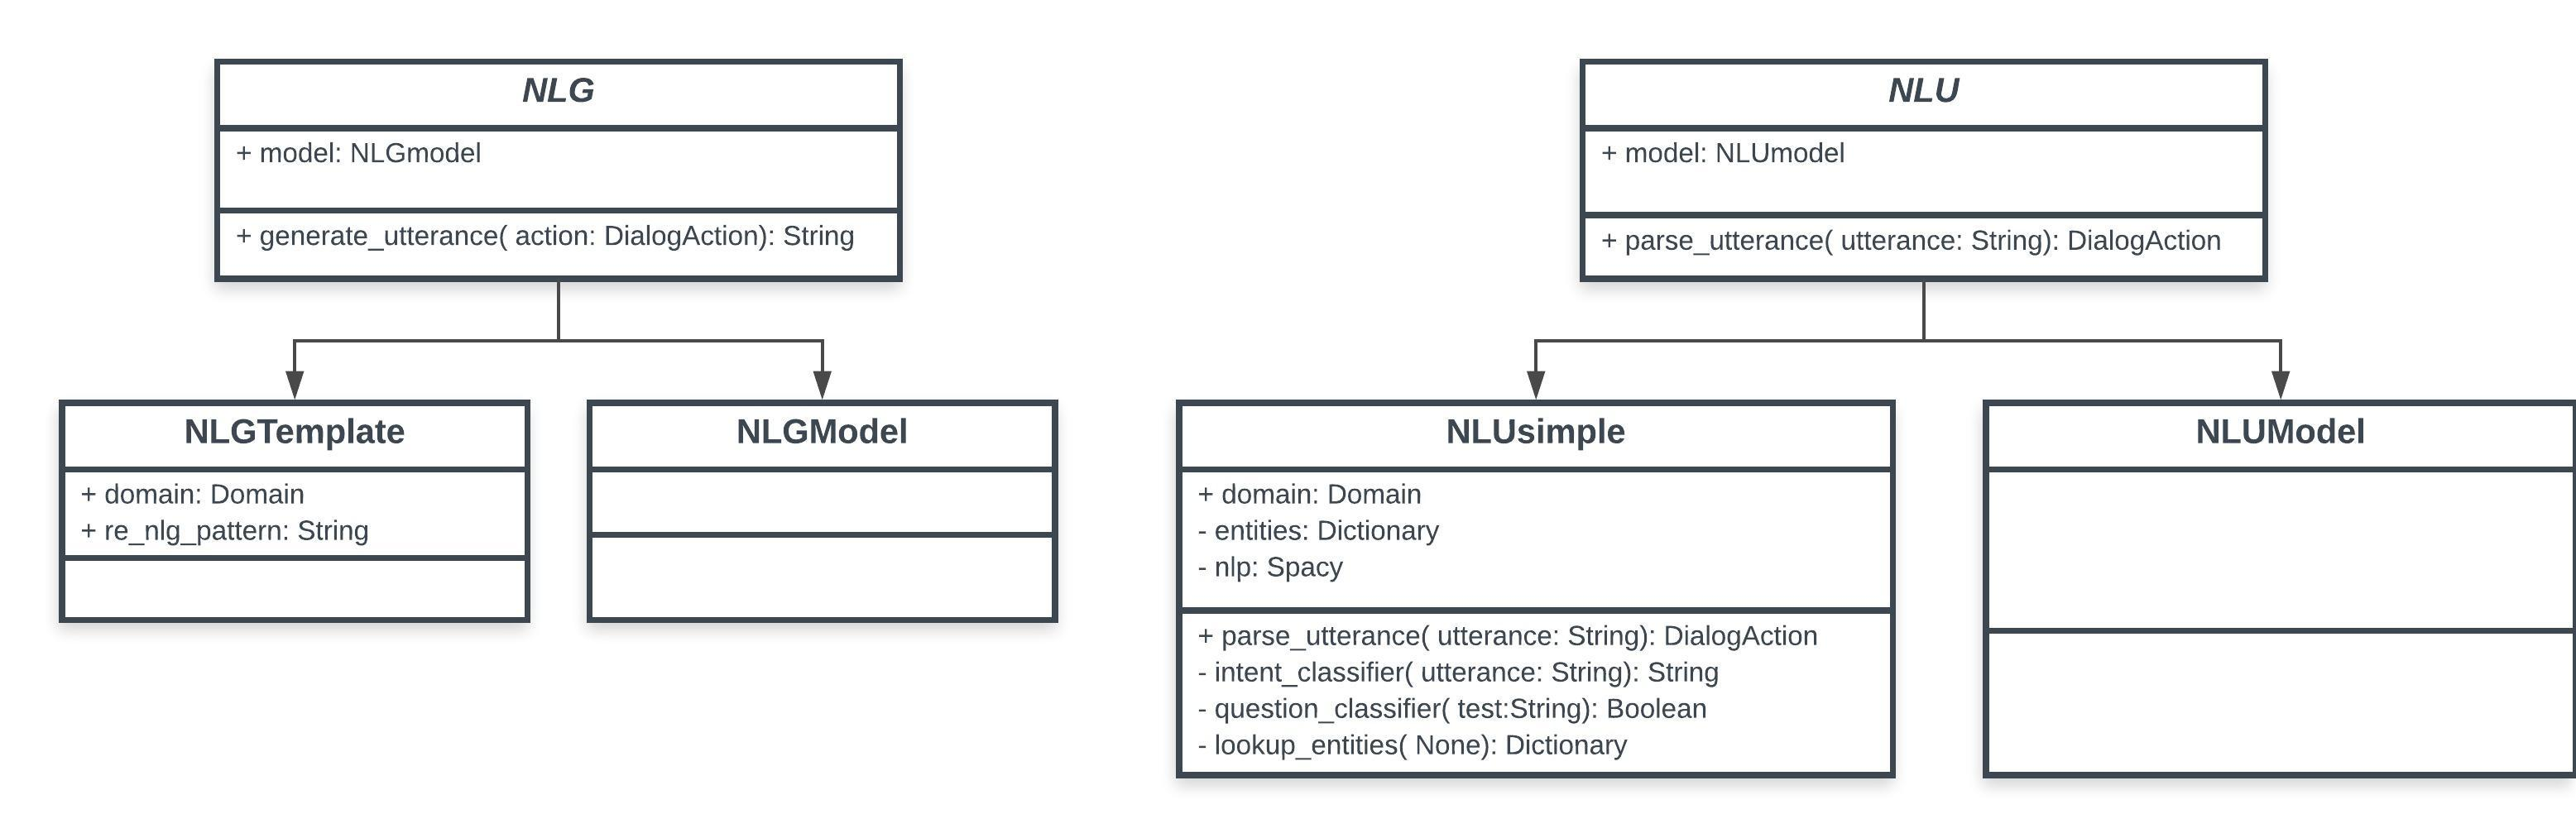
\includegraphics[ scale=.6]{diagrams/speaker_interface.jpeg}
	\caption{ NLU and NLG abstract base classes.}
	\label{fig:nlg_nlu}
\end{figure}

The NLU and NLG interface provides a common API for parsing and generating speech utterances for each speaker. Both interfaces define a single public-facing API method: \textit{parse utterance} and \textit{get utterance} respectively. \textit{Parse utterance} will take in a natural language speech utterance and return a \textit{DialogAction} object. \textit{Get utterance} takes in a dialog action and returns a natural language speech utterance.

The researcher has flexibility in setting up the NLU and NLG back-ends. In the implementation section, we will further detail the simple rules-based approach and neural machine translation implementations for both the nlg and nlu back-ends. 

Upon initialization, the speaker class will set an internal nlg and nlu object. The speaker's\textit{ get\_utterance } and \textit{parse\_utterance} will directly call the correspond methods in the nlg and nlu object. This way the dialog manager does not need to know the internals of each speaker's nlg and nlu objects. 

Nlu and nlg are open problem spaces and there are no universal solutions. In abstracting the nlu and nlg interfaces, the researcher has more flexibility in training and experimenting with their dialog agent. Since the user simulator will always return the machine-readable dialog action with the generated speech utterance, the researcher has the ability to train the nlu for their dialog agent to support more robust NLU use cases. 

\section{Dialog  Manager}

\begin{figure}[h!]
	\centering
	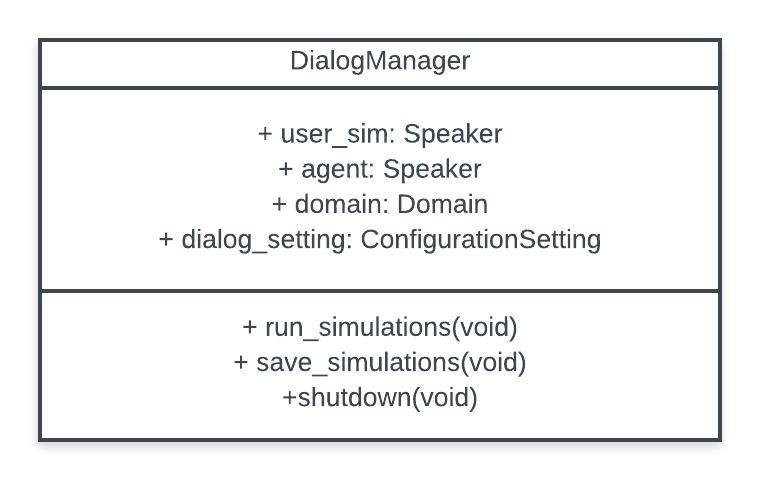
\includegraphics[ scale=1]{diagrams/dialog_manager.jpeg}
	\caption{ Dialog manager class. }
	\label{fig:dialog_manager}
\end{figure}

The dialog manager is the primary engine of the simulation framework. Its responsibilities include loading the dialog domain, setting up user simulator and dialog agent, running the simulations, and performing post-simulation metrics. The dialog manager does not need to be modified by the researcher and is set up to implement the researcher's simulations via a configuration file. The configuration file is translated into a configuration object by the command line tool and sent to the dialog manager. In the configuration file, the user specifies the following:
\begin{itemize}
	\item user simulator class
	\item dialog agent class
	\item dialog domain representation
	\item domain knowledge base class
	\item simulation settings 
\end{itemize}

The dialog manager uses Python dynamic loading capabilities to import the end user custom classes for the user simulator, dialog agent, and domain knowledge base. Once these are loaded into memory, the simulator runs the simulations. Figure 
\ref{fig:dialog_model} shows at a high level what the dialog model looks like. 
\begin{figure}[h!]
	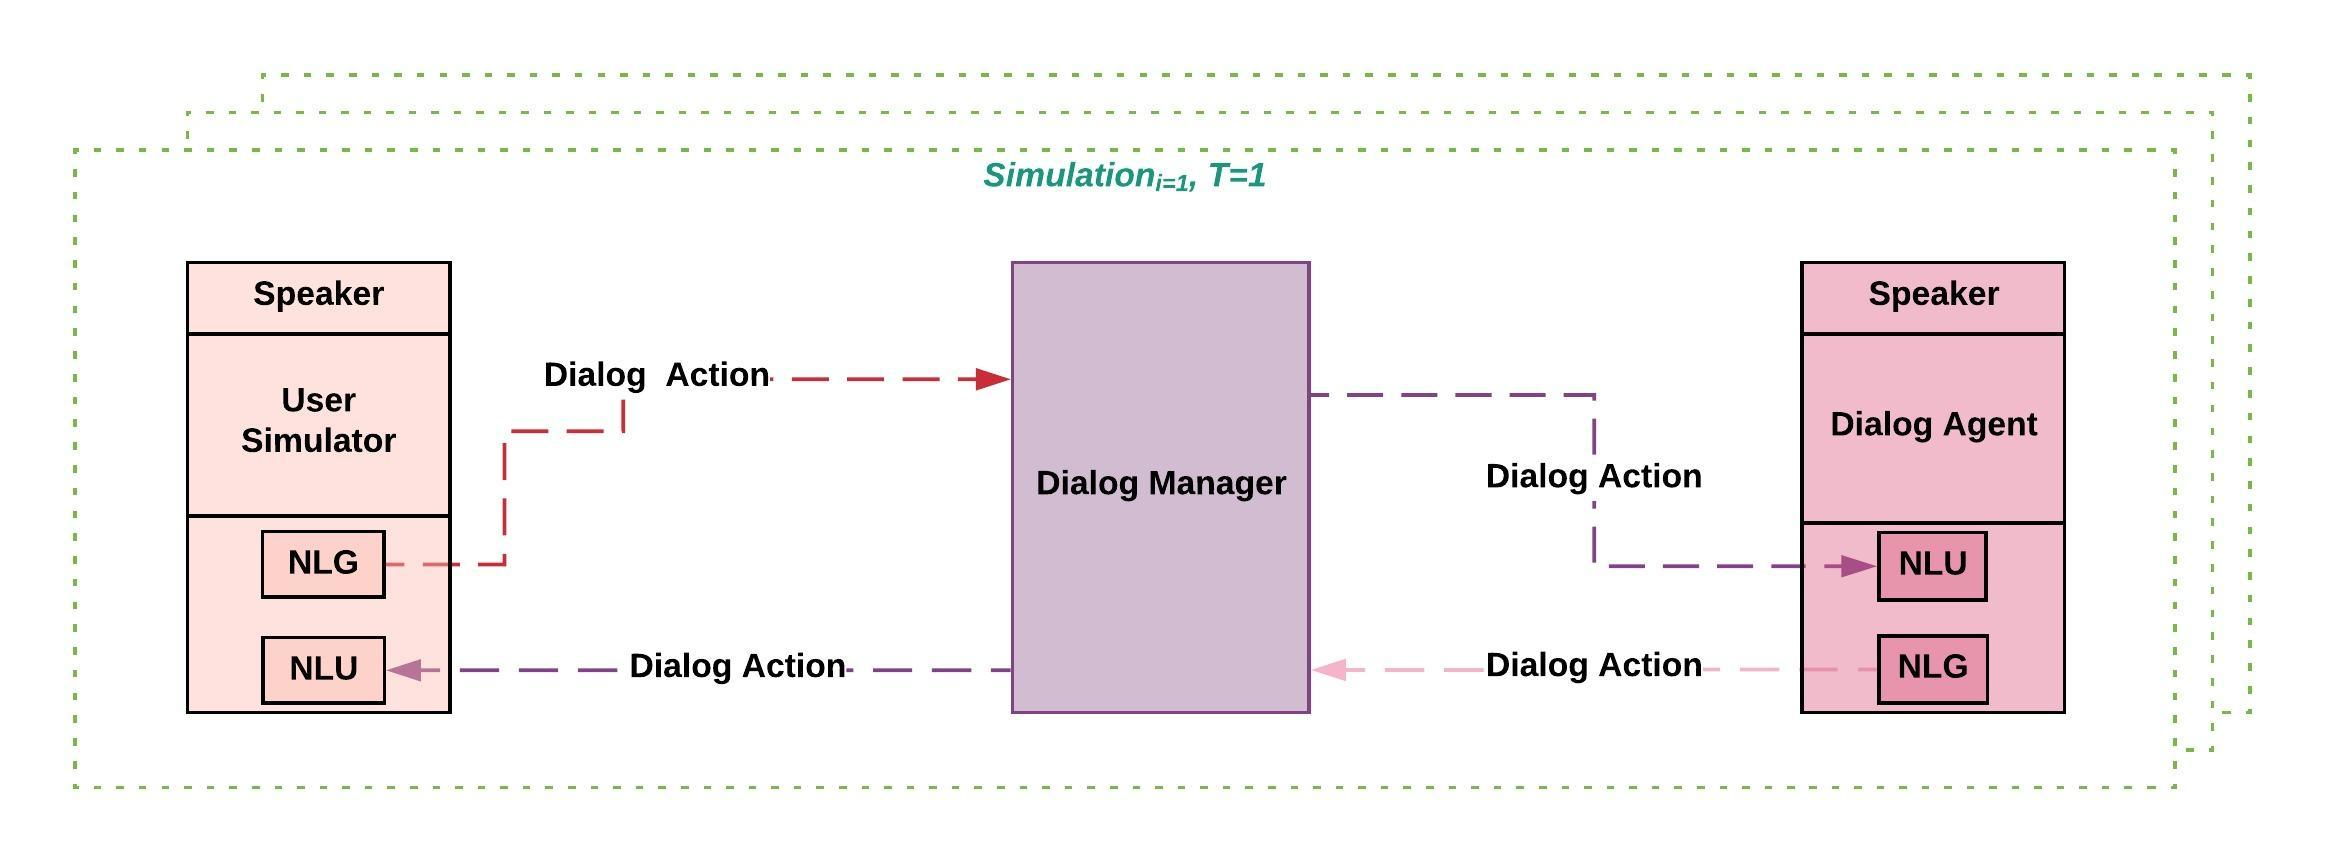
\includegraphics[width=\linewidth]{diagrams/dialog_model.jpeg}
	\caption{ Dialog model overview. }
	\label{fig:dialog_model}
\end{figure}

The dialog manager follows a basic pattern when running the simulation. It first generates a user goal, which will drive the user's hidden agenda and behavior. Next, it resets the user simulator with the newly generated goal and calls the dialog agent to reset itself. Once both speakers are ready to interact, the simulation is initiated. The logic for conversation is quite straightforward. The speaker class has the next method, which takes in dialog action and returns a response dialog action. The logic for the speakers to communicate with each other can be expressed in two lines (see Figure \ref{fig:conv_round}). The dialog action object standardizes how the speakers talk to each other and detail can be found below.  

Finally, in order to simulate a real user, the researcher can configure the user simulator to be corrupted in different ways. The user can change their minds and have a new preference generated from the dialog domain. To simulate faulty technical issues, the user may randomly exit the conversation. And finally, the user's goals can be corrupted resulting in an indiscernible signal from the user as to whether their goals were met or not. All these corruptions are specified by the researcher with a probability value, which represents the likelihood the user simulator will act aberrantly. This behavior will 
help generate more diverse data by providing negative examples.

\begin{figure}[h!]
	\label{fig:conv_round}
	\begin{lstlisting}
	# Assuming user speaks first 
	# 1. User Simulator takes turn and speaks
	user_action = user_simulator.next(previous_agent_action, turn_number)
	# 2. Agent takes turn and responds to user 
	agent_action = agent.next(previous_user_action, turn_number)
	\end{lstlisting}
	\caption{Pseudo code for conversation round.}
\end{figure}

Once all the simulations are run, the dialog simulator will run performance metrics to evaluate the efficacy of the dialog agent. If the user simulator was able to fill all the request slots in their hidden goal, the dialog is marked as successful. The researcher will be informed the average success rate of the dialog agent and can also see the round level evaluations in the generated dataset. After all simulations have been run, the dialog manager will serialize the output (if specified by the researcher) and exit. The goal of the output file is to provide quality annotated data that can be used as training data for supervised learning or reinforcement learning based dialog agent. 



%%% Local Variables: 
%%% mode: latex
%%% TeX-master: "main"
%%% End: 
